% kappa.tex
% ======================================================================

% Kappa class and personal tweaks
\documentclass[a4paper]{kappa}
\makeatletter
\setlength{\textwidth}{170mm}
\setlength{\columnsep}{1cm}  % increase space betweem columns
\setlength{\@figureindent}{0cm}  % remore figure caption padding
\makeatother

% load packages
\usepackage{amsmath}
\usepackage{bibentry}
\usepackage{bm}
\usepackage[T1]{fontenc}
\usepackage{natbib}
\usepackage{physics}
\usepackage[colorlinks, citecolor=blue]{hyperref}
\usepackage[sort]{cleveref}  % needs to be loaded after hyperref
\usepackage{doi}  % needs to be loaded after hyperref
\usepackage{graphicx}
\usepackage{multicol}
\graphicspath{{figures/}}
\nobibliography*

% Move floats to the end
%\usepackage[nolists]{endfloat}
%\renewcommand{\efloatseparator}{\mbox{}}

% Copernicus-style internal references
\crefname{chapter}{Chap.}{Chaps.}
\crefname{equation}{Eq.}{Eqs.}
\crefname{figure}{Fig.}{Figs.}
\crefname{section}{Sect.}{Sects.}
\crefname{table}{Table}{Tables}

% My commands
%\newcommand{\renote}[1]{\footnote{\textbf{Comment reply}: #1}}
\newcommand{\todo}[1]{} %\emph{[\textbf{Todo:} #1]}}
%\newcommand{\mref}[0]{\textbf{[ref.]}}

% Copernicus-like vertical space in tables
\newcommand\tophline{\hline\noalign{\vspace{1mm}}}
\newcommand\middlehline{\noalign{\vspace{1mm}}\hline\noalign{\vspace{1mm}}}
\newcommand\bottomhline{\noalign{\vspace{1mm}}\hline}

% Vectors and tensors
\newcommand{\vect}[1]{\va*{#1}} % bold arrow vectors
\newcommand{\tens}[1]{\vb*{#1}} % bold tensors

% Differential operators
\renewcommand{\div}[1]{\mathrm{div}\,#1}            % divergence
\renewcommand{\grad}[1]{\vect{\mathrm{grad}}\,#1}   % gradient
\newcommand{\tdiv}[1]{\vect{\mathrm{div}}\,#1}      % tensor divergence
\newcommand{\tgrad}[1]{\tens{\mathrm{grad}}\,#1}    % tensor gradient
\newcommand{\matdv}[1]{\pdv{#1}{t}+\vect{v}\cdot\grad{}\,#1}  % material dv.

% Common notations
\newcommand{\doteps}[0]{\dot{\epsilon}} % epsilon dot
\newcommand{\IDT}[0]{\tens{\delta}}     % Identity tensor
\newcommand{\CST}[0]{\tens{\sigma}}     % Cauchy stress tensor
\newcommand{\DST}[0]{\tens{\tau}}       % deviatoric stress tensor
\newcommand{\SRT}[0]{\tens{\doteps}}    % strain-rate tensor
\newcommand{\vv}[0]{\vect{v}}           % velocity vector
\newcommand{\vsia}[0]{\vv_{\mathrm{SIA}}}   % SIA velocity
\newcommand{\vssa}[0]{\vv_{\mathrm{SSA}}}   % SSA velocity
\newcommand{\PDD}[0]{\mathrm{PDD}}
\newcommand{\sPDD}[0]{\sigma_{\mathrm{PDD}}}

% Common units
\newcommand{\e}[1]{\ensuremath{\times 10^{#1}}}
\newcommand{\chem}[1]{\ensuremath{\mathrm{#1}}}
\newcommand{\unit}[1]{\ensuremath{\mathrm{#1}}}
\newcommand{\degree}[0]{\ensuremath{^{\circ}}}
\newcommand{\degC}[0]{\unit{{\degree}C}}

% Papers of the thesis
\newcommand{\CCLI}[0]{Paper~I}      % Cordillera climate
\newcommand{\PSDV}[0]{Paper~II}     % PDD SD variability
\newcommand{\PSDP}[0]{Paper~III}    % PDD SD parametrisation
\newcommand{\CCYC}[0]{Paper~IV}     % Cordillera cycle

% Github links
\newcommand{\issue}[1]{\href{https://github.com/pism/pism/issues/#1}{\##1}}

% Text label over graphics
% from http://tex.stackexchange.com/questions/128844/put-subfigure-labels-
% inside-figures-using-subfig-package
\newcommand{\subgraphics}[3][,]{%
  \setbox1=\hbox{\includegraphics[#1]{#3}}% Store image in box
  \leavevmode\rlap{\usebox1}% Print image
  \rlap{\hspace*{0.25em}
        \raisebox{\dimexpr\ht1-3ex}{\textbf{(#2)}}}% Print label
  \phantom{\usebox1}% Insert appropriate spacing
}

% Some general low-priority todos
% -- switch to kappa.cls
% -- incorporate figs as pdf, rasterize heavy elements
% -- use latex in matplotlib figures
% -- homogeneize subfig label fonts
% -- add software references
% -- redraw PISM interface

% Document properties
%\title{Numerical modelling of the Cordilleran ice sheet}
%\author{Julien Seguinot}
\thesistitle{Numerical modelling of the Cordilleran ice sheet}
\runningtitle{Numerical modelling of the Cordilleran ice sheet}
\candidate{Julien Seguinot}
\runningauthor{J. Seguinot}
\pubyear{2014}
\department{Department of Physical Geography and Quaternary Geology}
\university{Stockholm University}
\printed{Universitetsservice US-AB, 2014.}
%\issn{}
%\isbn{}
%\coverpic{Richard Swan. \textsf {www.richardswan.com}. Back cover portrait: Louise Tränk.}
%\layout{Summary and Papers IV \& V: Alistair Auffret based on  \LaTeX~templates by Rickard Petterson. Published papers typeset by respective publishers, reprinted with permission. Graphics created using \textsf{Inkscape}, \textsf{R} and \textsf{OpenOffice Draw}.}

% ======================================================================
\begin{document}
% ======================================================================

\begin{frontmatter}

\begin{abstract}

This doctoral thesis presents a study of the glacial history of northwestern
North America using numerical ice sheet modelling calibrated against field
evidence. The area is characterized by the steep topography of several mountain
ranges separated by large inter-montane depressions that were once covered by a
large-scale ice mass, the former Cordilleran ice sheet. Due to this complex
topographic setting, the Cordilleran ice sheet remains the least understood
Pleistocene ice sheet in terms of its extent, volume, and dynamics. Because of
the irregular topography on which the ice sheet formed, field studies have
often only had local or regional relevance. Numerical modelling, on the other
hand, allows quantitative reconstructions of whole ice sheet evolution based on
approximated physics of glacier flow.

This thesis presents simulations performed with PISM, a numerical ice sheet
model that approximates glacier flow by basal sliding and internal deformation,
and allows simulations of ice sheet growth and decay over multi-millenial time
scales. Sensitivity experiments have shown that simulations adopting climate
forcing from the North American Regional Reanalysis (NARR) yield ice sheet
extents that best fit the field constraints during the Last Glacial Maximum
(LGM). These simulations show that the geometry of the LGM Cordilleran ice
sheet can be largely explained by present-day temperature and precipitation
fields combined with palaeo-climate reconstructions if an accurate treatment of
seasonality, orographic precipitation, and daily temperature variability is
included in the ice sheet model.

In contrast to this short-lived, maximum ice sheet configuration, most of the
last glacial cycle is characterized by an intermediate state of glaciation
including isolated glaciers and ice caps covering the major mountain ranges of
the North American Cordillera. The largest and most persistent of these ice
sheet nucleation centres is located over the Skeena Mountains. Modelled
deglaciation conditions broadly match field evidence, and where they diverge,
such as over the Fraser Plateau, they indicate either a lack of important
processes in the model, or a more complex glaciation history than previously
thought. The model yields a readvance of the ice sheet during late glacial
times, which appears to match field evidence, before final retreat towards the
Skeena Mountains, which we identify as a key area to understanding glacial
dynamics of the Cordilleran ice sheet, highlighting the need for further
geological investigation of this region.

The simulations presented in this thesis demonstrate the potential of numerical
ice sheet modelling to inform on ice sheet history over glacial cycles,
provided that ice sheet models can be calibrated against field constraints.

\end{abstract}

%\begin{keyword}
%\end{keyword}
%\begin{svabstract}
%\end{svabstract}

\begin{thepapers}

\textbf{List of papers}

This doctoral dissertation consists of a cover summary and the following
journal articles, which are referred to by their Roman numerals in the text.

\begin{paper}
  \item \bibentry{Seguinot.etal.2014}.
  \item \bibentry{Seguinot.2013}.
  \item \bibentry{Seguinot.Rogozhina.2014}.
  \item \bibentry{Seguinot.etal.manuscript}.
\end{paper}

\vfill

\noindent\textbf{Author contributions}
\footnotesize{\begin{paper}
  \item[I] A.~P.~Stroeven initiated the Cordilleran ice sheet modelling
project; I set-up the ice sheet model (PISM) and supercomputing workflow, ran
simulations and wrote the first draft; C.~Khroulev implemented necessary code
changes in the model; I.~Rogozhina contributed to experiment design; A.~P.~Stroeven
helped with interpretation of the results; and Q.~Zhang prepared some of the
forcing data. All co-authors contributed to improve the text.
  \item[II] I analysed the weather data, wrote the positive degree day model
(PyPDD), ran computations and wrote the manuscript. A.~P.~Stroeven contributed
with editorial comments at the pre-submission stage and I.~Rogozhina helped to
assess the reviews.
  \item[III] I.~Rogozhina provided the original idea; I analysed the weather
data and developed a new parameterization of daily temperature standard
deviation. I.~Rogozhina and I wrote the manuscript. A.~P.~Stroeven contributed
with editorial comments at the pre-submission stage.
  \item[IV] I integrated the new parameterization of standard deviation into
PISM, ran the simulations and wrote the first draft; I.~Rogozhina guided
experiment design; A.~P.~Stroeven, M.~Margold and J.~Kleman took part in the
interpretation and comparison of model results against geological evidence. All
co-authors contributed to improve the text.
\end{paper}}

\end{thepapers}

\end{frontmatter}

\onecolumn

% ======================================================================
\hfill \textbf{\huge Cover summary}
\vfill
\tableofcontents
% ======================================================================

\newpage

\begin{figure*}[b]
  \centering
  \makebox[0pt]{
    \subgraphics{a}{photo-glacier-crevasses}
    \hspace{1cm}
    \subgraphics{b}{photo-glacier-susitna}
    \hspace{1cm}
    \subgraphics{c}{photo-glacier-fold}
  }
  \caption{Illustration of various glacier ice behaviours:
           \textbf{(a)} surface crevasses formed by ice flow over a hidden
           bedrock knob, Glacier Blanc, French Alps, 2004;
           \textbf{(b)} medial moraines illustrating downhill ice flow on
           Susitna Glacier, Alaska Range, photo by Austin Post, 1970
           \citep{NSIDC.2009}; and
           \textbf{(c)} mountain glacier calving into a small lake, revealing a
           folded structure formed by deformed debris layers in the ice,
           Glacier d'Arsine, French Alps, 2004.}
  \label{fig:glacier-mechanics}
\end{figure*}

\begin{figure*}[b]
  \centering
  \makebox[0pt]{
    \subgraphics{a}{photo-glacial-valley}
    \hspace{1cm}
    \subgraphics{b}{photo-erratic-boulder}
    \hspace{1cm}
    \subgraphics{c}{photo-melt-channels}
  }
  \caption{Different indicators of past glaciation:
           \textbf{(a)} glacial valley, exhibiting a broad, U-shaped profile
           characteristic of erosion by glaciers,
           Cirque du Fer-\`{a}-Cheval, French Alps, 2013;
           \textbf{(b)} erratic boulders, deposited in an improbable
           configuration as the glacier melted underneath,
           Finse area, Norwegian Scandes, 2011; and
           \textbf{(c)} lateral meltwater channels, formed on a gentle slope
           as the ice margin retreated towards the valley bottom, Tuya Lake
           area, Canadian Cordillera, 2012.}
  \label{fig:glaciation-indicators}
\end{figure*}

\begin{multicols}{2}  % appears necessary for bottom figures on first page

% ======================================================================
\section{Introduction}
% ======================================================================

In our daily life, we most commonly experience ice as small, solid cubes
that crackle on contact with refreshing liquids. Yet, on geological
time scales, and under high pressure, ice behaves quite differently.
In the cold and mountainous regions of the globe, ice accumulates through
cumulative snowfall until it reaches a critical thickness. Beyond this
threshold, usually in excess of 50\,m, but dependent on temperature, ice
deforms under its own weight to flow downhill (\cref{fig:glacier-mechanics}).
\emph{Glaciers}, these bodies of moving ice, move by a combination of
meltwater-induced sliding at the base \citep[\S532]{Saussure.1786},
and viscous deformation within the
ice body \citep{Forbes.1846b}.

As glaciers flow and slide across their bed, they transport
rock debris and erode the landscape, thereby leaving geomorphological traces of
their former presence (\cref{fig:glaciation-indicators}). In several parts of
the world, montane people
and early explorers learned since long to read these traces, and to
understand that glaciers had once been more extensive than today
\citep[e.g.,][p.~21]{Windham.Martel.1744}. With the emergence of the glacial
theory came the idea that, under colder temperatures
than today, expansive \emph{ice sheets} had once covered much of Europe and
North America \citep{Agassiz.1840}.

However, the glacial theory did not gain general acceptance until the
discovery and exploration
of the two present-day ice sheets on Earth, the Greenland and
Antarctic ice sheets, provided a modern analogue for the proposed European and
North American ice sheets. The first traverse of Greenland was performed by
Nansen in 1888, while Amundsen reached the south pole in 1911. Meanwhile, in
the European Alps, it was then discovered from observations of the glacial
landscape, that there had not been only one, but at least four, \emph{glacial
periods} \citep{Penck.Bruckner.1909}.

\end{multicols}
\twocolumn

More recently, palaeoclimate records extracted from deep sea sediments and ice
cores have provided a much more detailed picture of the Earth environmental
history \citep[e.g.,][]{Emiliani.1955, Shackleton.Opdyke.1973,
Dansgaard.etal.1993, Augustin.etal.2004}, indicating neither one, nor four, but
rather tens of glacial cycles. During the last 800000 years (800\,ka), glacial
and interglacial periods have succeeded each other with a 100\,ka periodicity
\citep[\cref{fig:paleo-timeseries};]{Hays.etal.1976, Augustin.etal.2004}.
However, much of the traces left by glaciers on the landscape date from the
most recent of these cycles, the \emph{last glacial cycle}.

\begin{figure}
  \centering
  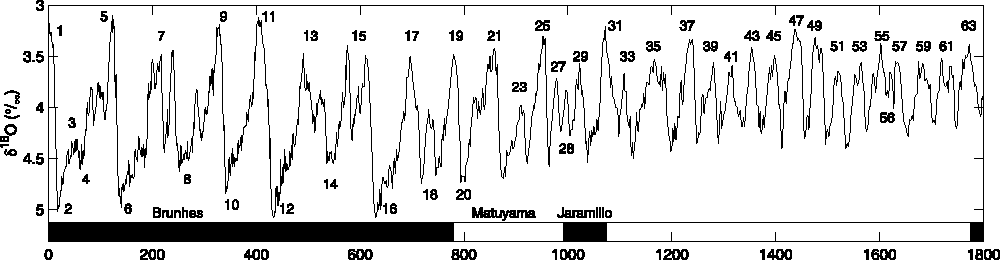
\includegraphics{paleo-timeseries}
  \caption{Palaeo-climate records of the last 800\,ka.
           \textbf{(a)} Benthic oxygen isotope (\chem{\delta^{18}O}) record
           from a compilation of globally-distributed deep sea sediment cores
           \citep{Lisiecki.Raymo.2005}. Higher \chem{\delta^{18}O} values
           correspond to periods of lower temperatures \citep{Emiliani.1955}
           or lower global sea level, and thus higher ice volume stored in
           glaciers and ice sheets on land \citep{Shackleton.1967}.
           \textbf{(b)} Temperature anomalies ($\Delta T$) reconstructed from a
           central Antarctic ice core \citep[EPICA Dome~C,][]{Jouzel.etal.2007}.
           The grey bands indicate the approximate time span of the last
           glacial period of 110 to 10\,ka.}
  \label{fig:paleo-timeseries}
\end{figure}

% ice volume 26.07 + 2.93 = 29.00
% metres sea-level 58.3 + 7.36 = 65.6
Together, the Greenland and Antarctic ice sheets currently host almost all
glacial ice on the planet, corresponding to 65.6\,m of potential sea level
rise, were these ice sheets to melt away entirely \citep{Bamber.etal.2013,
Fretwell.etal.2013}. At the apogee of the last glacial period, global sea level
was 120 to 135\,m lower than today
\citep{Clark.Mix.2002}, implying an additional, double amount of ice stored in
ice sheets and glaciers on land. Systematic mapping and compilation of glacial
landforms from all continents \citep[e.g.,][]{Prest.etal.1968,
Boulton.Clark.1990, Kleman.etal.1997, Hattestrand.1998} permitted
reconstructions of these former ice covers \citep{Ehlers.Gibbard.2007},
indicating that the excess ice volume
was repartitioned between more extensive Greenland and Antarctic ice sheets,
the Fennoscandian and Barents-Kara ice sheets in the Eurasian Arctic, and the
Innuitian, Laurentide, and \emph{Cordilleran} ice
sheets over North America (\cref{fig:paleo-glaciation}).

\begin{figure}
  \centering
  \includegraphics{paleo-glaciation}
  \caption{Spatial extent of ice sheet and glacier cover in the northern
           hemisphere \textbf{(a)} at present \citep{Patterson.Kelso.2014}, and
           \textbf{(b)} during the last glacial maximum
           \citep{Ehlers.Gibbard.2007}.}
  \label{fig:paleo-glaciation}
\end{figure}

Nevertheless, the landform record is sparse in time and, most often, spatially
incomplete. Palaeo-ice sheets did not leave a continuous imprint on the
lanscape, and much of this evidence has been overprinted by subsequent glacier
re-advances and other geomorphological processes \citep{Kleman.1994,
Kleman.etal.2006, Kleman.etal.2010}.
Therefore, geomorphological reconstructions of former glacier extent require a
substantial amount of interpretation. This is where numerical ice sheet models,
incorporating the processes of glacier sliding \citep[e.g.,][]{Weertman.1957}
and deformation \citep[e.g.,][]{Nye.1953} observed on modern glaciers, can
help. Although these models alone contain too many uncertainties to reproduce
accurate ice sheet reconstructions during former glacial cycles
\citep[e.g.,][]{Hebeler.etal.2008}, they can be calibrated against geological
data where they exist \citep{Napieralski.etal.2007}, while allowing
physics-based, quantitative reconstructions of ice sheet sectors where they do
not \citep[e.g.,][]{Marshall.etal.2002, Tarasov.Peltier.2004}.

\begin{figure*}
  \centering
  \makebox[0pt]{\includegraphics{map-northamerica}}
  \caption{Relief map of northern North America showing a reconstruction of the
           areas covered by the Cordilleran (CIS), Laurentide (LIS), Innuitian
           (IIS) and Greenland (GIS) ice sheets during the last glacial maximum
           \citep[21.4 to 16.8\,cal\,\chem{^{14}C}\,kyr\,BP,][]{Dyke.2004}.
           The rectangular box delimits the model domain used in all simulation
           and most figures of this thesis. The background
           map consists of ETOPO1 \citep{Amante.Eakins.2009} and Natural Earth
           Data \citep{Patterson.Kelso.2014}.}
  \label{fig:map-northamerica}
\end{figure*}

In addition, numerical ice sheet models provide quantitative insights on the
four-dimensional distribution of stresses and deformations in palaeo-ice sheets
and allow for reconstructions of their past thickness and volume evolution, which
are difficult to infer from geological evidence.

In this thesis, I focus on numerical modelling of the last Cordilleran ice
sheet, which once covered much of the mountainous terrain of western North
America \citep{Dawson.1888}, a region where topographic complexity has
presented a particular challenge to reconstructing glacial history based on the
geomorphological record \citep[e.g.,][]{Kleman.etal.2010} or numerical ice
sheet modelling \citep{Robert.1991}.


% ======================================================================
\section{North American Cordillera}
% ======================================================================

During the last glacial cycle, much of North America has been covered by ice
(\cref{fig:map-northamerica}). During the Last Glacial Maximum (LGM), peak of
glaciation, three major ice sheets had collided to
form a continuous blanket of ice that spanned from southern Alaska to
Newfoundland, connecting with the Greenland ice sheet in the Canadian Arctic,
and extending as far south as Chicago.
The Laurentide ice sheet, largest of the three, was centred on the Hudson Bay,
and fully covered the Canadian Prairies, Eastern Canada, and the Great Lakes
Basin. The Innuitian ice sheet, much smaller, covered the northernmost Canadian
archipelago. Finally, the \emph{Cordilleran ice sheet}, intermediate in size,
capped the mountain
ranges of the Western Cordillera.

\begin{figure*}
  \centering
  \makebox[0pt]{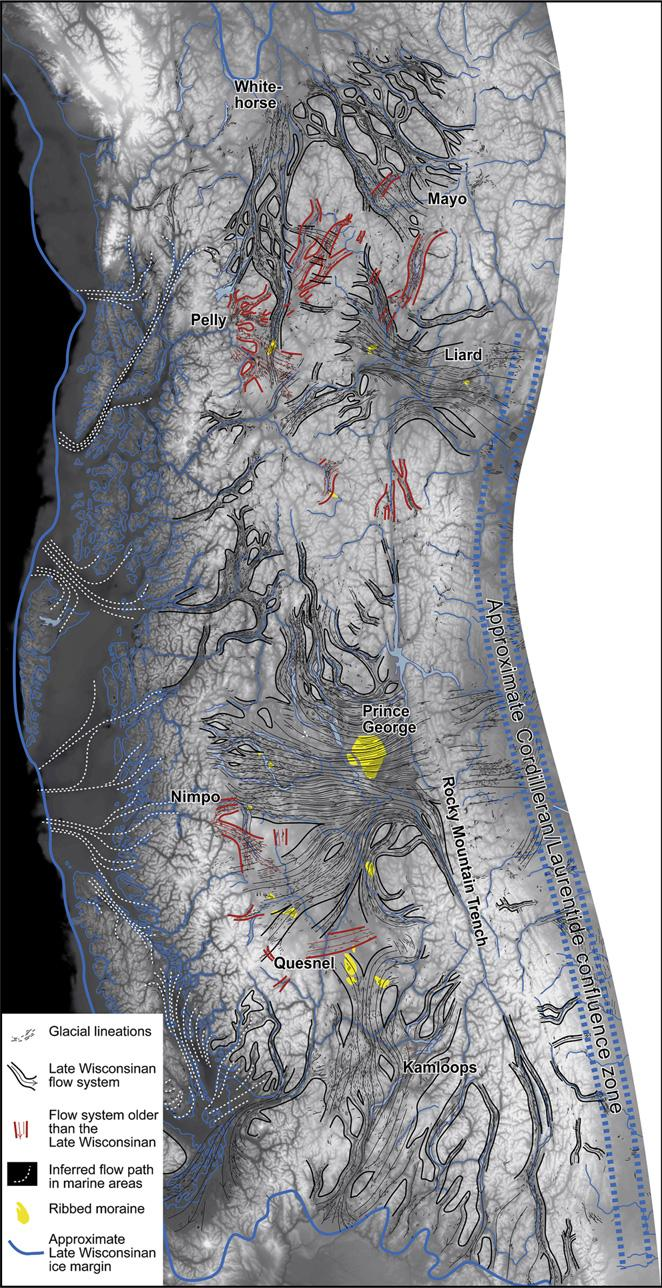
\includegraphics{map-cordillera}}
  \caption{Topographic map of the northern American Cordillera, oriented north.
           Cumulative last glacial maximum ice cover \citep{Dyke.2004} is
           marked in red, and the model domain in black.
           The background map consists of ETOPO1 \citep{Amante.Eakins.2009}
           and Natural Earth Data \citep{Patterson.Kelso.2014}.}
  \label{fig:map-cordillera}
\end{figure*}

\begin{figure*}
  \centering
  \makebox[0pt]{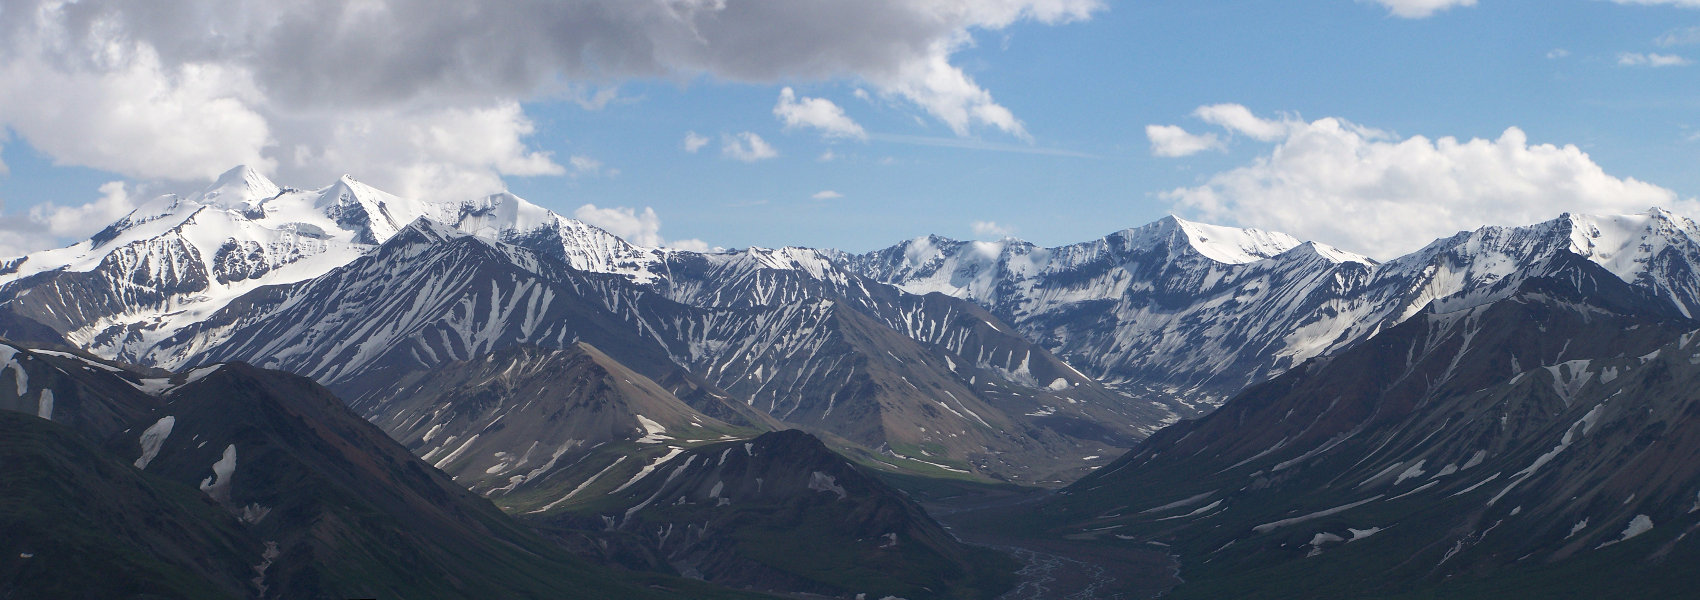
\includegraphics{photo-alaska-range}}
  \caption{The Alaska Range hosts several of the highest peaks in the North
           American Cordillera. Despite this fact and its northerly location,
           its north slope hosts relatively small glaciers only, which had not
           been much more extensive during the Last Glacial Maximum
           \citep{Kaufman.Manley.2004}, indicating dry climatic conditions.
           The Alaska Range is tectonically active and rapidly eroding, as
           shown by landslide-covered valley sides on this photograph.}
  \label{fig:photo-alaska-range}
\end{figure*}

\begin{figure*}
  \centering
  \makebox[0pt]{
    \subgraphics{a}{photo-vancouver-island}
    \hspace{1cm}
    \subgraphics{b}{photo-fraser-valley}
  }
  \caption{Contrasted climates of the North American Cordillera:
           \textbf{(a)} Pacific Coast at Vancouver Island, western British
           Columbia, by Martin Margold, 2010.
           \textbf{(b)} Fraser Valley, south-central British Columbia, 2010.}
  \label{fig:photo-fraser-valley}
\end{figure*}

% ----------------------------------------------------------------------
\subsection{Topographic setting}
% ----------------------------------------------------------------------

The North American Cordillera forms an elongated but broad mountain system with
an average east-west width of about 1000\,km (\cref{fig:map-cordillera}). Its
topography is a complex jigsaw of mountain ranges and interior basins. It was
formed during multiple accretion phases associated with the closure of several
back-arc oceanic trenches, over a 200 million year (200\,Ma)-long geological
history \citep{Sigloch.Mihalynuk.2013}.

The \emph{dominant reliefs} occur along two major ribbons that run parallel to
each other along the general orientation of the North American Cordillera. The
western ribbon is formed by the Pacific Coast orogenic belt and includes, from
north to south, the Alaska Range (\cref{fig:photo-alaska-range}), the Wrangell
and Saint-Elias Mountains,
the Coast Mountains and the North Cascades. The eastern ribbon consists of the
Nevadan and Laramide belts, which are separated by the deep and strikingly
linear Rocky Mountain / Tintina Trench depression, and includes the Selwyn and
MacKenzie Mountains in the north, and the Rocky mountains in the south. The
Brooks Range of northern Alaska has been covered by ice, but its glaciers
remained disjunct from the main body of the Cordilleran ice sheet
\citep{Kaufman.Manley.2004}.

\todo{Go to geolibrary and check \emph{Geology of Canada} books and such for a
      reference about the three orogenic belts.}

The North American Cordillera hosts several \emph{intermontane basins}, the
presence
of which influenced former patterns of Cordilleran ice sheet flow. The two
major depressions are the Fraser Plateau in south-central British Columbia, and
the Liard Lowland in northern British Columbia (\cref{fig:map-cordillera}).
These two basins are separated by the Skeena Mountains, a mildly elevated, but
extensive and deeply incised mountain group. This is the most dominant upland
area in-between the dominant topographic ribbons that form the North American
Cordillera.

The ubiquitously mountainous topography of the region presents a serious
obstacle to reconstructing the palaeoglaciology of the Cordilleran ice sheet.
Because of the irregular arrangement of valleys and ridges that formed the ice
sheet's subglacial landscape, ice moved along tortuous and intertwined
pathways, sometimes following the major topographical troughs, and sometimes
flowing across them \citep{Davis.Mathews.1944, Kleman.etal.2010}. In terms of
numerical ice sheet modelling, the presence of steep and irregular subglacial
topography yields complex flow patterns and stress distributions within the ice
sheet and requires high-resolution and thus, large computational grids.

% ----------------------------------------------------------------------
\subsection{Climatic setting}
% ----------------------------------------------------------------------

\begin{figure*}
  \centering
  \makebox[0pt]{\includegraphics{plot-atm}}
  \caption{Some characteristics of the Cordilleran climate according to the
           North American Regional Reanalysis
           \citep[NARR,][]{Mesinger.etal.2006}.}
  \label{fig:plot-atm}
\end{figure*}

The topographic complexity of the North American Cordillera is associated with
distinctive patterns of temperature and precipitation, whose effects on
vegetation are clearly expressed in the landscape
(\cref{fig:photo-fraser-valley}). Due to the large latitudinal extent of the
region, mean annual \emph{temperatures} vary significantly from north to south
(\cref{fig:plot-atm}a). About half of the model domain has mean annual
temperatures below freezing. However, temperature \emph{seasonality},
here computed as the difference between the warmest and the coldest months,
varies between around 10\,\degC\ along most of the Pacific Coast to above
40\,\degC\ for the interior Arctic sectors
(\cref{fig:plot-atm}b). There exists a
partial correlation between cold regions and those that have a large
seasonality, so that many regions where mean annual temperatures are well below
freezing point experience warm summers.

Annual \emph{precipitation rates} are highest on the western slopes of the
Pacific Coast ranges and decline quickly on the eastern side of the mountains
(\cref{fig:photo-fraser-valley,fig:plot-atm}c). In terms of ice sheet
mass balance, this contrast is even reinforced through the differences in
\emph{timing of maximum precipitation} through the year (\cref{fig:plot-atm}d).
Coastal regions receive most precipitation during fall and winter, which is
therefore largely delivered as snow. In contrast, many inland regions
experience dry winters, and most of the annual precipitation, consequently
falls there as rain during summer, further enhancing ice melt.

These topographically-induced, spatial variations in temperature and
precipitations tightly constrain the location of potential ice sheet nucleation
centres that lead to the formation of a Cordilleran ice sheet. The numerical
ice sheet model is therefore highly sensitive to the choice of input topography
and climate used (\cref{sec:atm}). This forms the motivation for the study
presented in \CCLI, where the climatic setting of the North American Cordillera
is also described in further detail.

% ----------------------------------------------------------------------
\subsection{Glacial history}
% ----------------------------------------------------------------------

Evidence from glaciofluvial deposits dated using cosmogenic nuclides at
$2.64^{+0.20}_{-0.18}$\,Ma (uncertainty range from 2.46 to 2.84\,Ma)
indicates the first presence of an ice sheet in the
Cordilleran mountains during the late Pliocene \citep{Hidy.etal.2013}.
This indicates that the North American Cordillera has been glaciated many times
since the late Pliocene, with the first of these glaciations occurring even
before the mid-Pleistocene onset of 100 ka glacial cycles
(\cref{fig:paleo-timeseries}). However, only fragments of the last few
glaciations can be reconstructed from the geologic record, implying that much
of the older evidence has been erased by subsequent glacial re-advances and
perhaps even by other, non-glacial geomorphological processes.

In the \emph{northern sector} of the Cordilleran ice sheet domain, at least
four glaciations have been identified
    \citep{Duk-Rodkin.1999, Ward.etal.2007, Ward.etal.2008,
           Briner.Kaufman.2008, Demuro.etal.2012,
           Stroeven.etal.2010, Stroeven.etal.2014}.
The two older ones, often collectively referred to as the Reid and pre-Reid
glaciations, pre-date the last glacial cycle, and are therefore beyond the
scope of this study. The two younger glaciations, however, occurred both during
the last glacial cycle. First, the older one of the two, the Gladstone
Glaciation,
reached its maximum extent between $50.4\pm3.0$ and $54.3\pm2.0\,^{10}$Be\,ka
\citep{Ward.etal.2007}, during Marine Oxygen Isotope Stage (MIS) 4, a period of
relatively large global ice volume. However, evidence from the Gladstone
Glaciation has not been documented along the southern ice sheet margin, making
it difficult to seize its spacial extent. The younger one of the two last
glacial
cycle glaciations, the McConnell Glaciation, is associated with end moraines of
oldest minimum apparent exposure ages of $15.7\pm1.5$ and
$17.7\pm1.6\,^{10}$Be\,ka \citep{Stroeven.etal.2014}, which appears to
correspond to the last global ice volume maximum (MIS~2). In contrast to the
Gladstone Glaciation, the McConnell Glaciation appears contemporaneous with
glacial advance of the southern ice sheet margin during the Fraser glaciation,
with a maximum extent attained between $17.4$ and
$16.4$\,\unit{^{14}C\,cal\,ka} \citep{Porter.Swanson.1998}. Within errors
inherent to the cosmogenic nuclide exposure dating methods
\citep{Heyman.etal.2011}, the McConnell and Fraser glaciations correspond to
the same glacial episode, which resulted in the LGM extent of the Cordilleran
ice sheet.

Apart from geological evidence of the final demise of the Cordilleran ice sheet, most field
evidence relates to its LGM extent. It indicates that ice covered most of the
Canadian Cordillera, and some of the adjacent regions in north-western
contiguous USA and Alaska (\cref{fig:map-cordillera}). The Cordilleran ice
sheet originated from the coalescence of several mountain-centred ice caps
\citep{Davis.Mathews.1944}. It is generally thought that this LGM configuration
was short-lived \citep{Clague.etal.1980, Clague.1985, Cosma.etal.2008}, a
hypothesis which can be studied through numerical modelling.

The \emph{southern margin} of the ice sheet has been studied extensively, and
is in several respects better understood than its northern counterpart
\citep{Booth.etal.2003}. It consists of coalescent piedmont lobes, each of
which formed at the outlet of the main valleys. The Puget Lobe
\citep{Thorson.1980, Porter.Swanson.1998} was the westernmost and largest one.
It covered the Puget Lowland, a region that comprises the cities of Vancouver
and Seattle. Further east, beyond the Cascade Range, the Okanagan and Purcell
lobes formed the southern Cordilleran ice sheet margin. The latter dammed
the Clark Fork River, inhibiting runoff and forming Glacial Lake Missoula
\citep{Pardee.1910}. As the ice sheet margin retreated, the lake repeatedly and
catastrophically drained to the Pacific Ocean \citep{Bretz.1923,Waitt.1980}.
These floods contributed to shape a distinctive landscape, known as the
Channeled Scabland.

The \emph{western margin} of the Cordilleran ice sheet covered part of the
Pacific continental shelf. An independent ice cap covering Vancouver Island
diverted flow from the main body of ice to drain into the Strait of Georgia
between Vancouver Island and the Olympic Peninsula, where it formed the Juan
de Fuca marine ice lobe, calving into the Pacific Ocean. Further to the
North, the ice margin encroached the Queen Charlotte Islands. However, the
archipelago may not have been fully ice-covered, even during the maximum of
glaciation. Submarine troughs traversing several portions of the continental
shelf indicate the erosional action of additional ice streams, yet it is not
clear whether they have formed during the last glacial cycle or during earlier
glaciations.

\todo{Find refs for marine extent of the ice sheet}

Finally, the conditions at the \emph{eastern margin} of the Cordilleran ice
sheet are the least understood. Although it is known that the Cordilleran ice
sheet collided with the Laurentide ice sheet at times during the last glacial
cycle \citep[e.g.][]{Margold.etal.2013, Margold.etal.2013a}, the nature of the
interaction between the two ice sheets and the precise location of this
junction remains unclear \citep{Gowan.2013}, while limited information exists
on its timing \citep[e.g.][]{Jackson.etal.1997, Bednarski.Smith.2007}. Because
the present thesis focuses specifically on the Cordilleran ice sheet, I,
therefore, neglect buttressing effects of the Laurentide ice sheet.

The retreat of the ice sheet during the last \emph{deglaciation} was likely
rapid. Most of the evidence for the style and pace of deglaciation comes from
the Fraser Plateau. Studies there have indicated that some of the highest
uplands emerged from the ice sheet prior to the surrounding lowlands, possibly
resulting in thin, stagnant ice remnants covering parts of the plateau
\citep{Fulton.1967, Fulton.1991, Margold.etal.2011, Margold.etal.2013a}. Less
is known about the deglaciation of the northern sector of the Cordilleran ice
sheet, but abundant glacial landforms from the Liard Lowland indicate a
different mode of deglaciation, with active retreat of the ice margin towards
the surrounding mountain ranges \citep{Margold.etal.2013}. Patterns of
deglaciation, as well as the possibility for a late-glacial re-advance, are
discussed in further detail and compared with modelling results in
\CCYC.

% ======================================================================
\section{Numerical ice sheet model}
% ======================================================================

% ----------------------------------------------------------------------
\subsection{Overview}
% ----------------------------------------------------------------------

The simulations presented in this thesis employ the \emph{Parallel Ice Sheet
Model} (PISM), an open-source, finite-difference, shallow ice sheet model
\citep{PISM-authors.2014}. The model requires bedrock topography, sea level,
geothermal heat flux and climate forcing as inputs, and computes the thermal
and dynamic states of the ice sheet, and the associated thermal and
deformational responses of an idealised lithosphere. However, the atmosphere
and ocean are not part of the model. Instead, PISM includes boundary models
that provide simple parametrisations of their interaction with the ice sheet
across interfaces that are assumed to be well defined
(\cref{fig:model-interfaces}).

This section does not attempt to provide an extensive description of PISM,
which can be found in an on-line documentation
\citep[\url{http://www.pism-docs.org},][]{PISM-authors.2014}.
Instead, it aims to highlight the modelling choices that I have made in this
thesis, and to present an overview of the physics involved in these choices.
Parameter values are summarised in \cref{tab:params}.

\begin{figure}
  \centering
  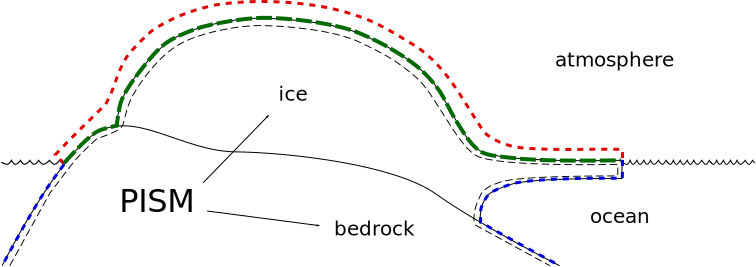
\includegraphics[width=85mm]{model-interfaces}
  \caption{PISM is a numerical model for ice and bedrock physics. Processes
           occurring at the interface with the atmosphere and the ocean, that
           are progressive transitions in nature, are parametrised along
           well-defined boundaries in the model.
           From \citet{PISM-authors.2014}.}
  \label{fig:model-interfaces}
\end{figure}

\begin{table*}
  \centering
  \caption{Constant parameters of the ice sheet model.}
  \label{tab:params}
  \makebox[0pt]{\begin{tabular*}{170mm}{@{\hspace{2em}}l@{\extracolsep{\fill}}lrll}
    \tophline
    Not.    & Name & Value & Unit & Source \\
    \middlehline

    \multicolumn{2}{l}{\emph{Ice material properties}} \\

    $\rho$  & Ice density
            & 910
            & \unit{kg\,m^{-3}}
            & \citet{Aschwanden.etal.2012} \\

    $g$     & Standard gravity
            & 9.81
            & \unit{m\,s^{-2}}
            & \citet{Aschwanden.etal.2012} \\

    $n$     & Glen exponent
            & 3
            & -
            & - \\

    $A_c$   & Ice hardness coefficient cold
            & 3.61\e{-13}
            & \unit{Pa^{-3}\,s^{-1}}
            & \citet{Paterson.Budd.1982} \\

    $A_w$   & Ice hardness coefficient warm
            & 1.73\e3
            & \unit{Pa^{-3}\,s^{-1}}
            & \citet{Paterson.Budd.1982} \\

    $Q_c$   & Flow law activation energy cold
            & 6.0\e4
            & \unit{J\,mol^{-1}}
            & \citet{Paterson.Budd.1982} \\

    $Q_w$   & Flow law activation energy warm
            & 13.9\e4
            & \unit{J\,mol^{-1}}
            & \citet{Paterson.Budd.1982} \\

    $R$     & Ideal gas constant
            & 8.31441
            & \unit{J\,mol^{-1}\,K^{-1}}
            & - \\

    $T_c$   & Flow law critical temperature
            & 263.15
            & \unit{K}
            & \citet{Paterson.Budd.1982} \\

    $f$     & Flow law water fraction coeff.
            & 181.25
            & -
            & \citet{Lliboutry.Duval.1985} \\

    $\beta$ & Clapeyron constant
            & 7.9\e{-8}
            & \unit{K\,Pa^{-1}}
            & \citet{Luthi.etal.2002} \\

    $c_i$   & Ice specific heat capacity
            & 2009
            & \unit{J\,kg^{-1}\,K^{-1}}
            & \citet{Aschwanden.etal.2012} \\

    $c_w$   & Water specific heat capacity
            & 4170
            & \unit{J\,kg^{-1}\,K^{-1}}
            & \citet{Aschwanden.etal.2012} \\

    $k$     & Ice thermal conductivity
            & 2.10
            & \unit{J\,m^{-1}\,K^{-1}\,s^{-1}}
            & \citet{Aschwanden.etal.2012} \\

    $L$     & Water latent heat of fusion
            & 3.34\e5
            & \unit{J\,kg^{-1}\,K^{-1}}
            & \citet{Aschwanden.etal.2012} \\

    \multicolumn{2}{l}{\emph{Basal sliding}} \\

    $q$     & Pseudo-plastic sliding exponent
            & 0.25
            & -
            & - \\

    $v_{th}$& Pseudo-plastic threshold velocity
            & 100.0
            & \unit{m\,yr^{-1}}
            & - \\

    $c_0$   & Till cohesion
            & 0.0
            & Pa
            & - \\

    $\alpha$& Effective pressure coefficient (\CCLI)
            & 0.95
            & -
            & - \\

    $\delta$& Effective pressure coefficient (\CCYC)
            & 0.02
            & -
            & - \\

    $e_0$   & Till reference void ratio
            & 0.69
            & -
            & \citet{Tulaczyk.etal.2000} \\

    $C_c$   & Till compressibility coefficient
            & 0.12
            & -
            & \citet{Tulaczyk.etal.2000} \\

    $W_{max}$ & Maximal till water thickness
            & 2.0
            & m
            & - \\

    $b_0$   & Altitude of max. friction angle
            & 0
            & m
            & - \\

    $b_1$   & Altitude of min. friction angle
            & 200
            & m
            & - \\

    $\phi_0$& Minimum friction angle
            & 10/15
            & \degree
            & - \\

    $\phi_1$& Maximum friction angle
            & 30/45
            & \degree
            & - \\

    \multicolumn{2}{l}{\emph{Bedrock and lithosphere}} \\

    $\rho_b$& Bedrock density
            & 3300
            & \unit{kg\,m^{-3}}
            & - \\

    $c_b$   & Bedrock specific heat capacity
            & 1000
            & \unit{J\,kg^{-1}\,K^{-1}}
            & - \\

    $k_b$   & Bedrock thermal conductivity
            & 3.0
            & \unit{W\,m^{-1}\,K^{-1}}
            & - \\

    $q_G$   & Geothermal heat flux
            & 70.0
            & \unit{mW\,m^{-2}}
            & - \\

    $\nu_m$ & Mantle viscosity
            & 1\e21
            & \unit{Pa\,s}
            & \citet{Lingle.Clark.1985} \\

    $\rho_l$& Lithosphere density
            & 3300
            & \unit{kg\,m^{-3}}
            & \citet{Lingle.Clark.1985} \\

    $D$     & Lithosphere flexural rigidity
            & 5.0\e24
            & \unit{N}
            & \citet{Lingle.Clark.1985} \\

    \multicolumn{2}{l}{\emph{Surface and atmosphere}} \\

    $T_0$   & Temperature of snow precipitation
            & 0.0
            & \degC
            & - \\

    $T_1$   & Temperature of rain precipitation
            & 2.0
            & \degC
            & - \\

    $F_s$   & Degree-day factor for ice
            & 3.04\e{-3}
            & \unit{m\,K^{-1}\,day^{-1}}
            & \citet{Shea.etal.2009} \\

    $F_i$   & Degree-day factor for ice
            & 4.59\e{-3}
            & \unit{m\,K^{-1}\,day^{-1}}
            & \citet{Shea.etal.2009} \\

    $\gamma$& Air temperature lapse-rate
            & 6\e{-3}
            & \unit{K\,m{-1}}
            & - \\

    \bottomhline
  \end{tabular*}}
\end{table*}

% ----------------------------------------------------------------------
\subsection{Field equations}
% ----------------------------------------------------------------------

The thermodynamic core of the ice sheet model relies on four elementary field
equations: the equation of incompressibility, the balance of stresses, the constitutive law for ice, and the conservation of energy. Firstly, ice flow is assumed \emph{incompressible}. Hence, ice
density, $\rho$, is constant, and
conservation of mass therefore implies a conservation of volume, which can be expressed
in terms of the ice velocity vector, $\vv$ (\cref{fig:model-variables}), by
\begin{equation}
    \label{eqn:incompressibility}
    \div{\vv} = 0 \,.
\end{equation}

\begin{figure}
  \centering
  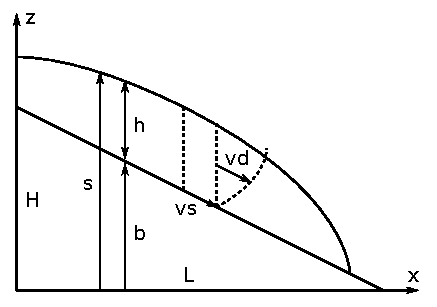
\includegraphics{model-variables}
  \caption{Sketch of notations used for the main variables of the ice sheet
           model. An infinitesimal ice parcel is moving at velocity $\vv$,
           under the balance of stresses $\CST$ and gravity $\vect{g}$.}
  \label{fig:model-variables}
\end{figure}

Secondly, the \emph{balance of stresses} is expressed by the Stokes equation,
thus assuming creeping flow. In other words, ice is considered as a slow-moving
fluid whose deformation is entirely controlled by internal friction, here
expressed by the Cauchy stress tensor, $\CST$, and the gravity vector,
$\vect{g}$:
\begin{equation}
    \label{eqn:stressbalance}
    \tdiv{\CST} + \rho\,\vect{g} = \vect{0} \,.
\end{equation}

Thirdly, after defining the strain-rate tensor
${\SRT = \frac{1}{2}(\tgrad{\vv} + \tgrad{\vv}^{\mathrm{T}})}$,
and the deviatoric stress tensor, ${\DST = \CST + p\,\IDT}$,
where $p=-\frac{1}{3}\tr(\CST)$ is the hydrostatic pressure and
$\tens{\delta}$ is the identity tensor, a \emph{constitutive law} for ice
\citep{Nye.1953} based on laboratory experiments \citep{Glen.1952} is used to
relate these two quantities. It reads:
\begin{equation}
    \label{eqn:glenslaw}
    \SRT = A\,\tau_e^{n-1}\,\DST \,.
\end{equation}
The equivalent stress, $\tau_e$, is defined by
${\tau_e}^2 = -\mathrm{II}_{\DST} = \frac{1}{2} \tr(\DST^2)$,
where $\mathrm{II}_{\DST}$ is the second invariant of the stress tensor.
The ice softness coefficient, $A$, depends on ice temperature, $T$, pressure, $p$, and
water content, $\omega$, through an Arrhenius-type law
\citep[Eqs.~63--65]{Paterson.Budd.1982, Aschwanden.etal.2012},
\begin{equation}
    A =
    \begin{cases}
        A_c (1+f\omega)\,e^\frac{-Q_c}{RT_{pa}}
            & \text{if}\ T < T_c \,, \\
        A_w (1+f\omega)\,e^\frac{-Q_w}{RT_{pa}}
            & \text{if}\ T \ge T_c \,,
    \end{cases}
\end{equation}
where $T_{pa}$ is the pressure-adjusted temperature calculated using the
Clapeyron relation, ${T_{pa} = T - \beta p}$. $R$ is the ideal gas constant,
and $A_c$, $A_w$, $Q_c$ and $Q_w$, are constant parameter corresponding to
values measured below and above a critical temperature threshold
${T_c=-10}$\,\degC\ \citep[\cref{tab:params};][]{Paterson.Budd.1982}.
The water fraction, $\omega$, is capped at a maximum value of 0.01, above which
no measurements are available \citep[Eq.~5.7]{Lliboutry.Duval.1985,
Greve.1997}.

For a convenient derivation of the shallow shelf approximation, developed in
the next section (\cref{sec:siassa}), the constitutive law can be rewritten
using an inverted formulation. Assuming
${{\doteps_e}^2 = \frac{1}{2} \tr(\SRT^2)}$ and ${B=A^{-1/n}}$,
\cref{eqn:glenslaw} becomes
\begin{equation}
    \label{eqn:invglenslaw}
    \DST = B\,\doteps_e^{(1/n)-1}\,\SRT \,.
\end{equation}

By analogy to Newtonian flow, an apparent viscosity, $\nu$, can then be defined
by ${\DST = 2 \nu\SRT}$, thus yielding
\begin{equation}
    \label{eqn:viscosity}
    \nu = \frac{B}{2}\,\doteps_e^{(1/n)-1} \,.
\end{equation}

Finally, the evolution of temperature within the ice is governed by the
\emph{conservation of energy}. In PISM, the conservation of energy uses an
enthalpy formulation in order to
account for thermodynamic effects associated with internal phase changes in the
glacier \citep[Eqs.~20--21]{Aschwanden.etal.2012}. This enthalpy ($H$)
formulation reads
\begin{equation}
    \label{eqn:enthalpy}
    \rho \left(\matdv{H}\right)
        = -\div{\vect{q}} + \frac{\nu\doteps_e^2}{4} \,,
\end{equation}
where $\vect{q}$ represents the heat flow and
${\nu\dot{\epsilon_e}^2/4 = \tr(\DST\SRT)}$ is a
source term corresponding to strain heat release. In the case where ice
temperature, $T$, is below the pressure-melting point, the heat flow is
modelled by Fourier's law, $\vect{q} = k\,\grad{T}$, where $k$ is the thermal
conductivity of ice, while enthalpy can be expressed as $H=c\,T$, where $c$
denotes the ice specific heat capacity (\cref{tab:params}).
Consequently, the enthalpy equation (\ref{eqn:enthalpy}) can be rewritten using
a more familiar, cold-ice, temperature formulation,
\begin{equation}
    \label{eqn:temperature}
    \matdv{T} = \frac{k}{\rho c} \Delta T
                + \frac{\nu\doteps_e^2}{4\rho c} \,.
\end{equation}
However, note that, here, the term ``enthalpy'' is actually an abuse of
language, commonly used in glaciology as a synonym of ``interval energy''
\citep{Aschwanden.etal.2012}.

\Cref{eqn:incompressibility,eqn:stressbalance,eqn:glenslaw,eqn:enthalpy}
constitute the thermodynamic basis
of the model. However, their resolution in full form implies a computational
demand too high for multi-millennial, continental-scale applications, such as
the numerical modelling of the Cordilleran ice sheet through the last 100\,ka
glacial cycle, thus requiring shallow approximations.


% ----------------------------------------------------------------------
\subsection{Shallow approximations}
\label{sec:siassa}
% ----------------------------------------------------------------------

PISM employs two well-documented
approximations of the ice flow equations: the shallow ice approximation (SIA)
and the the shallow shelf approximation (SSA). Although both approximations can
be derived from a rigorous scaling approach
    \citep{Morland.Johnson.1980, Hutter.1983,
           Morland.1987, Weis.etal.1999},
I won't expand these lengthy derivations
here, assuming instead the simplifications and focusing on their effect.

Distinguishing the hydrostatic and deviatoric components of the stress tensor,
the balance of stresses (\ref{eqn:stressbalance}) can be expanded into
\begin{equation}
    \tdiv{\DST} - \grad{p} + \rho\,\vect{g} = \vect{0} \,.
\end{equation}

Projecting along the three Cartesian axes, this reads
\begin{subequations}
\label{eqn:fullstokes}
\begin{align}
    \pdv{\tau_{xx}}{x} + \pdv{\tau_{xy}}{y} + \pdv{\tau_{xz}}{z}
        &= \pdv{p}{x} \,, \\
    \pdv{\tau_{yx}}{x} + \pdv{\tau_{yy}}{y} + \pdv{\tau_{yz}}{z}
        &= \pdv{p}{y} \,, \\
    \pdv{\tau_{zx}}{x} + \pdv{\tau_{zy}}{y} + \pdv{\tau_{zz}}{z}
        &= \pdv{p}{z} - \rho g \,.
\end{align}
\end{subequations}

The \emph{shallow ice approximation} (SIA) assumes that basal friction is high
enough
for the vertical shear stresses $\{\tau_{xz}, \tau_{yz}\}$ to predominate over
all other components of the deviatoric stress tensor. In this framework, the
projected stress-balance can be simplified to
\begin{subequations}
\label{eqn:sia}
\begin{align}
    \label{eqn:siax}
    \pdv{\tau_{xz}}{z} &= \pdv{p}{x} \,, \\
    \label{eqn:siay}
    \pdv{\tau_{yz}}{z} &= \pdv{p}{y} \,, \\
    \label{eqn:siaz}
    0 &= \pdv{p}{z} - \rho g \,.
\end{align}
\end{subequations}

\todo{\citet{Morland.Johnson.1980} derived the SIA in 2D, using a stream
      function. Their equations look very different from here. Go to
      geolibrary and check the book by \citet{Hutter.1983}, if it is there.}

Neglecting atmospheric pressure, \Cref{eqn:siaz} yields the pressure,
\begin{equation}
    p = \rho g (s-z) \,,
\end{equation}
varying from zero at the ice surface, $s$, to $\rho gh$ at the base, ${b=s-h}$
(\cref{fig:model-variables}). This expression
can be re-introduced into \cref{eqn:siax,eqn:siay}, thus yielding the
expression of the horizontal shear stresses, sometimes referred to as driving
stresses,
\begin{subequations}
\begin{align}
    \tau_{xz} &= -\rho g (s-z) \pdv{s}{x} \,, \\
    \tau_{yz} &= -\rho g (s-z) \pdv{s}{y} \,.
\end{align}
\end{subequations}

Using the constitutive law (\ref{eqn:glenslaw}), vertical derivatives of
horizontal velocities can be related to the horizontal shear stresses:
\begin{subequations}
\begin{align}
    \pdv{v_x}{z} &= 2A (\tau_{xz}^2 + \tau_{yz}^2)^{n-1} \tau_{xz} \,, \\
    \pdv{v_y}{z} &= 2A (\tau_{xz}^2 + \tau_{yz}^2)^{n-1} \tau_{yz} \,.
\end{align}
\end{subequations}

Thus, within the framework of the SIA, horizontal velocities $\vv_{SIA}$ can be
directly expressed as a function of the slope gradient,
\begin{subequations}
\begin{align}
    \pdv{v_x}{z} &= -2A (\rho g)^n (s-z)^n
                    \left(\pdv{s}{x}+\pdv{s}{y}\right)^{n-1} \pdv{s}{x} \,, \\
    \pdv{v_y}{z} &= -2A (\rho g)^n (s-z)^n
                    \left(\pdv{s}{x}+\pdv{s}{y}\right)^{n-1} \pdv{s}{y} \,,
\end{align}
\end{subequations}
which yields, in vectorial notation,
\begin{equation}
    \label{eqn:vsia}
    \pdv{\vsia}{z} = -2A\,(\rho g)^n\,(s-z)^n\,|\grad{s}|^{n-1}\,\grad{s} \,.
\end{equation}

From \cref{eqn:vsia} it can be seen that shallow ice velocities, $\vsia$,
can be directly computed from the geometry of the ice sheet surface, $s$,
after a single vertical integration over the ice thickness, in order to
account for variations of ice rheology, $A$, with depth.

\todo{If I have time, show that vertical velocities can be
      obtained from the compressibility equation.}

The \emph{shallow shelf approximation} (SSA), in contrast to SIA, assumes that
basal friction is low enough for ice to deform uniformly within the entire ice
column. In this context, the stress-balance can
be simplified to \citep[Eqs.~4.10--4.12]{Weis.etal.1999}
\begin{subequations}
\label{eqn:ssa}
\begin{align}
    \label{eqn:ssax}
    \pdv{\tau_{xx}}{x} + \pdv{\tau_{xy}}{y} + \pdv{\tau_{xz}}{z}
        &= \pdv{p}{x} \,, \\
    \label{eqn:ssay}
    \pdv{\tau_{yx}}{x} + \pdv{\tau_{yy}}{y} + \pdv{\tau_{yz}}{z}
        &= \pdv{p}{y} \,, \\
    \label{eqn:ssaz}
    \pdv{\tau_{zz}}{z} &= \pdv{p}{z} - \rho g \,,
\end{align}
\end{subequations}
and horizontal velocities can be assumed independent of depth
\citep[Eq.~4.22]{Weis.etal.1999}, so that
\begin{align}
    \pdv{v_x}{z} &= 0 \,, \\
    \pdv{v_y}{z} &= 0 \,.
\end{align}

Once again neglecting atmospheric pressure, and remembering that $\tr(\DST)=0$,
\Cref{eqn:ssaz} yields the pressure
\begin{align}
    p &= \rho g (s-z) + \tau_{zz} \,, \\
      &= \rho g (s-z) - \tau_{xx} - \tau_{yy} \,,
\end{align}
which can be re-introduced into \cref{eqn:ssax,eqn:ssay}:
\begin{subequations}
\begin{align}
    2\pdv{\tau_{xx}}{x} + \pdv{\tau_{yy}}{x} + \pdv{\tau_{xy}}{y}
        + \pdv{\tau_{xz}}{z} &= \rho g \pdv{s}{x} \,, \\
    \pdv{\tau_{yx}}{x} + 2\pdv{\tau_{yy}}{y} + \pdv{\tau_{xx}}{y}
        + \pdv{\tau_{yz}}{z} &= \rho g \pdv{s}{y} \,.
\end{align}
\end{subequations}

Using the inverse formulation of the constitutive law \eqref{eqn:invglenslaw},
components of the deviatoric stress tensor can be replaced by corresponding
velocity components, yielding
\begin{subequations}
\begin{gather}
  \begin{split}
    \pdv{x} \left[2\bar{\nu}
                  \left(2\pdv{v_x}{x} + \pdv{v_y}{y}\right) \right]
        &+ \pdv{y} \left[\bar{\nu}
                         \left(\pdv{v_x}{y} + \pdv{v_y}{x}\right) \right] \\
        &+ \pdv{\tau_{xz}}{z} = \rho g \pdv{s}{x} \,,
  \end{split}\\
  \begin{split}
    \pdv{x} \left[\bar{\nu}
                  \left(\pdv{v_x}{y} + \pdv{v_y}{x}\right) \right]
        &+ \pdv{y} \left[2\bar{\nu}
                         \left(\pdv{v_x}{x} + 2\pdv{v_y}{y}\right) \right] \\
        &+ \pdv{\tau_{yz}}{z} = \rho g \pdv{s}{y} \,,
  \end{split}
\end{gather}
\end{subequations}
where $\bar{\nu}$ is the depth-integrated apparent viscosity defined by
\begin{equation}
    \bar{\nu} = \frac{1}{H}\int_b^s\nu \,.
\end{equation}

A final integration over the entire ice column yields
\citep[Eqs.~7.7--7.8]{Weis.etal.1999}
\begin{subequations}
\begin{gather}
  \label{eqn:vssa}
  \begin{split}
    \pdv{x} \left[2\bar{\nu}h
                  \left(2\pdv{v_x}{x} + \pdv{v_y}{y}\right) \right]
        &+ \pdv{y} \left[\bar{\nu}h
                         \left(\pdv{v_x}{y} + \pdv{v_y}{x}\right) \right] \\
        &+ \tau_{bx} = \rho gh \pdv{s}{x} \,,
  \end{split}\\
  \begin{split}
    \pdv{x} \left[\bar{\nu}H
                  \left(\pdv{v_x}{y} + \pdv{v_y}{x}\right) \right]
        &+ \pdv{y} \left[2\bar{\nu}h
                         \left(\pdv{v_x}{x} + 2\pdv{v_y}{y}\right) \right] \\
        &+ \tau_{by} = \rho gh \pdv{s}{y} \,,
  \end{split}
\end{gather}
\end{subequations}
where $\tau_{bx}$ and $\tau_{by}$ correspond to $x$ and $y$-components of the
basal traction, and will be determined by a sliding law.

In contrary to the the SIA velocities, $\vsia$, the SSA velocities, $\vssa$,
can not be computed in a direct manner. Instead, \cref{eqn:vssa} must be
resolved numerically using iteration methods, in order to obtain
approximated values for $\vssa$.

In PISM, the SIA and SSA velocities are eventually added
\citep[\cref{fig:model-siassa};][Eq.~15]{Winkelmann.etal.2011}:
\begin{equation}
    \label{eqn:siassa}
    \vv = \vsia + \vssa \,.
\end{equation}
Because $\vsia$ is small where $\vssa$ is large, and
reciprocally, we can expect the model to perform well in regions where
conditions for applicability of either the SIA or the SSA are met
(\cref{fig:model-siassa}). However,
\cref{eqn:siassa} is a heuristic, and its validity in the zone of
transition between shear flow (SIA) and longitudinal flow (SSA) has not been
mathematically proven.

\begin{figure}
  \centering
  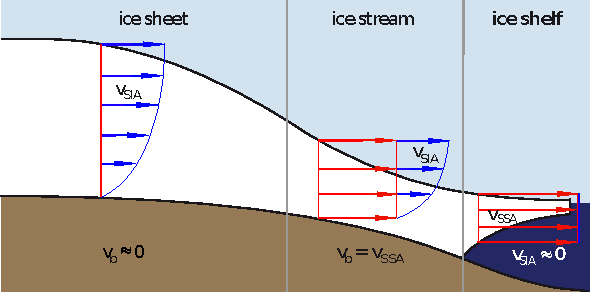
\includegraphics[width=80mm]{model-siassa}
  \caption{Combination of Shallow Ice Approximation (SIA) and Shallow Shelf
           Approximation (SSA) velocities in PISM, assuring a smooth transition
           between shear-dominant and longitudinal stress regimes. After
           \citet[Fig.~1]{Winkelmann.etal.2011}. Not to scale.}
  \label{fig:model-siassa}
\end{figure}


% ----------------------------------------------------------------------
\subsection{Basal sliding}
% ----------------------------------------------------------------------

Although the SIA is valid only under non-sliding conditions, the SSA requires
a sliding law as basal boundary condition, which in fact constitutes the main
control on SSA velocities and, in turn, the locations of ice streams in the
model.

The simulations presented here use a \emph{pseudo-plastic} sliding law,
\begin{equation}
    \label{eqn:pseudoplastic}
    \vect{\tau}_b = -\tau_c \frac{\vv_b}{{v_{th}}^q\,|\vv_b|^{1-q}} \,,
\end{equation}
where $\vect{\tau}_b$ is the basal traction force, $\vv_b$ is the basal
velocity, and $v_{th}$ is an arbitrary velocity threshold
(\cref{tab:params}). Note that, in the case of
$q=0$, \cref{eqn:pseudoplastic} corresponds to a purely plastic law
\citep[Eq.~11]{Winkelmann.etal.2011},
\begin{equation}
    \label{eqn:plastic}
    \vect{\tau}_b = -\tau_c \frac{\vv_b}{|\vv_b|} \,.
\end{equation}

The yield stress $\tau_c$ is related to till properties by the Mohr-Coulomb
criterion,
\begin{equation}
    \label{eqn:coulomb}
    \tau_c = c_0 + N\,\tan{\phi} \,.
\end{equation}

The till cohesion $c_0$ is assumed to be zero.
The effective pressure on the
till, $N$, is determined by the modelled amount of water at the bed. However,
two different parametrisations are used within this thesis. In {\CCLI}, using
PISM~0.5, the effective pressure is linearly related to water content by a
simple parametrisation \citep[Eq.~13]{Winkelmann.etal.2011},
\begin{equation}
    N = \rho gh (1 - \alpha \frac{W}{W_{max}}) \,,
\end{equation}
where $W$ is the amount of water at the bed, and varies from zero to
$W_{max}=2$\,m, a threshold above which further melt simply exits the system,
thus assuming instantaneous drainage. Although mass-conserving water drainage
is now implemented in PISM \citep{Bueler.Pelt.2014}, it is not included in the
simulations presented here for the sake of simplicity.

In {\CCYC}, using PISM~0.6, the effective pressure is determined by an
empirical parametrisation based on laboratory experiments on Antarctic till
\citep{Tulaczyk.etal.2000, Bueler.Pelt.2014},
\begin{equation}
    N = \delta \rho gh \, 10^{(e_0/C_c) (1 - (W/W_{max}))} \,,
\end{equation}
where $e_0$ is a measured reference void ratio, $C_c$ a measured
compressibility coefficient, and $\delta$ is a non-dimensional parameter
chosen as 0.02 based on simple sensitivity tests on the Greenland ice sheet
(Table~\ref{tab:params}).

Finally, the till friction angle, $\phi$ (\cref{eqn:coulomb}), is taken as a
function of modern bed
elevation, with lowest values occurring at low elevations, thus accounting for
a weakening of till associated with the presence of marine sediments
\citep[cf.][Eq.~10]{Martin.etal.2011},
\begin{equation}
    \phi(x,y) =
    \begin{cases}
        \phi_0 & \text{if}\ b \le b_0 \,, \\
        \phi_0 + (\phi_1-\phi_0) \frac{b - b_0}{b_1-b_0}
                & \text{if}\ b_0 < b < b_1 \,, \\
        \phi_1 & \text{if}\ b_1 \le b \,,
    \end{cases}
\end{equation}
where $b_0=0$\,m is modern sea-level and $b_1=200$\,m is a rough average of
highest observed palaeo-shoreline elevations in the model domain
\citep[\cref{tab:params};][]{Clague.James.2002}.


% ----------------------------------------------------------------------
\subsection{Bedrock response}
% ----------------------------------------------------------------------

The modelled ice sheet interacts with the underlying bedrock in two ways.
Firstly, \emph{bedrock temperatures} are computed to a given depth by
appending the
ice enthalpy model (\ref{eqn:enthalpy}) with an underlying bedrock thermal
model. The only process accounted for is vertical heat conduction, hence this model
consists of a simple diffusion equation,
\begin{equation}
    \pdv{T}{t} = \frac{k_b}{\rho_b c_b} \Delta T \,,
\end{equation}
where $k_b$, $\rho_b$ and $c_b$ are the thermal conductivity, density and
specific heat capacity of the bedrock (\cref{tab:params}).
Bedrock temperature is conditioned at depth by a fixed upwards geothermal heat
flux $q_G$  (\cref{tab:params}). The bedrock thermal model
is necessary for modelling the Cordilleran ice sheet on multi-millennial
time-scales, because temperature fluctuations caused by climate change and
varying degrees of isolation from atmospheric temperatures by ice sheet
coverage, penetrate several kilometres
into the rock, and eventually affect basal ice temperatures.

Secondly, bedrock elevation evolves in response to the ice weight. The
\emph{bedrock deformation} model used in this thesis describes the flexure of
an elastic
lithosphere on top of an infinite half-space viscous mantle
\citep{Lingle.Clark.1985}. It can be described by a single pseudo-differential
equation of the bed elevation, $b$,
\begin{equation}
    \label{eqn:beddef}
    2\nu_m\,|\grad|\,\pdv{b}{t} + \rho_l g b + D\,\Delta^2 b = \sigma_{zzb} \,,
\end{equation}
where $\nu_m$ is mantle viscosity, $\rho_l$ is lithosphere density, $D$ is the
lithosphere's flexural rigidity (\cref{tab:params}), and $\sigma_{zzb}$
corresponds to the ice load
\citep{Bueler.etal.2007}. Here, ${\Delta^2 = (\div\grad{})^2}$ designs the
biharmonic (Laplacian square) operator of
linear elastic theory, while $|\grad{}|$ is a pseudo-differential operator
defined through its Fourier transform by \citet[Eq.~6]{Bueler.etal.2007}. On
the left-hand side of \cref{eqn:beddef}, the first term accounts for mantle
relaxation, the second for point-wise isostasy, and the third for elastic
flexure. Due to high mantle viscosity, $\nu_m$, there exists a time lag between
the ice sheet growth and the isostatic bedrock response.


% ----------------------------------------------------------------------
\subsection{Surface mass balance}
% ----------------------------------------------------------------------

At the interface between the ice sheet and the atmosphere
(\cref{fig:model-interfaces}),
surface mass fluxes are computed from monthly mean surface air temperature,
$T_m$, and monthly precipitation, $P_m$, using a temperature-index model
\citep[\cref{fig:model-pdd}; cf.][]{Hock.2003}. Snow accumulation, $A_s$,
equals precipitation
when temperature is below ${T_0=0\,\degC}$, and decreases to zero
linearly with temperature between $T_0$ and ${T_1=2\,\degC}$,
\begin{equation}
    A_s =
    \begin{cases}
        P_m     & \text{if}\ T_m \le T_0 \,, \\
        P_m \frac{T_1-T_m}{T_1-T_0}
                & \text{if}\ T_0 < T_m < T_1 \,, \\
        0       & \text{if}\ T_1 \le T_m \,,
    \end{cases}
\end{equation}

Surface melt, $M$, is assumed proportional to the number of positive degree
days (PDD), defined over an arbitrary time interval, $[t_1, t_2]$, as the
integral of positive Celcius temperature $\theta = T-T_0$,
\begin{equation}
    \mathrm{PDD} = \int_{0}^{A}\max(\theta(t),0)\,dt \,.
\end{equation}

For multimillenial simulations of palaeo-ice sheet evolution such as
presented in this thesis, daily or hourly temperature data is not available,
forcing the PDD computation to rely on an idealised representation of the
annual temperature cycle $\theta_{ac}$. Sub-annual temperature variability around
the freezing point, however, significantly affects surface melt on a multi-year
scale \citep{Arnold.Mackay.1964}. It is then typically included in the models
under an assumption of normal temperature distribution, using a standard
deviation parameter $\sPDD$ in the PDD computation \citep{Braithwaite.1984}.
PDDs can then be computed using a double-integral formulation
\citep{Reeh.1991},
\begin{multline}
    \PDD = \frac{1}{\sPDD\sqrt{2\pi}} \\
        \times
        \int_{t_1}^{t_2} \mathrm{d}t
        \int_{0}^{\infty} \mathrm{d}\theta \,
        \theta \exp\left({-\frac{(\theta-\theta_{ac})^2}{2\sPDD^2}}\right) \,,
\end{multline}
or more efficiently using an error function formulation
\citep{Calov.Greve.2005},
\begin{multline}
    \label{eqn:calovgreve}
    \PDD = \int_{t_1}^{t_2} \mathrm{d}t
        \bigg[\frac{\sPDD}{\sqrt{2\pi}}
                \exp\left({-\frac{\theta_{ac}^2}{2\sPDD^2}}\right) \\
              + \frac{\theta_{ac}}{2} \, \mathrm{erfc}
                \left(-\frac{\theta_{ac}}{\sqrt{2}\sPDD}\right)\bigg] \,.
\end{multline}

In the simulations presented here, \cref{eqn:calovgreve} is numerically
approximated using week-long sub-intervals. For each sub-interval, PDDs, which
serve as a proxy for the available energy for melt, define the amount of snow
melt through a proportionality factor $F_s$. If all snow is melted, remaining
PDDs are then used to melt ice, using a proportionality factor $F_i$
(\cref{fig:model-pdd}). The degree-day factors for snow, $F_s$, and ice, $F_i$
(\cref{tab:params}),
are derived from mass-balance measurements on contemporary glaciers in the
Coast and Rocky mountains of British Columbia \citep{Shea.etal.2009}. In
{\CCLI}, the temperature standard deviation $\sPDD$ is a constant model
parameter. In {\CCYC}, it is computed from daily temperature values from the
North American Regional Reanalysis \citep[NARR,][]{Mesinger.etal.2006}, using
a method initially developed in {\PSDV}, and further improved upon in {\PSDP}.
Although the PDD model is a crude parametrisation of processes happening at the
surface of a glacier, its applicability has been demonstrated
\citep[e.g.][]{Hock.2003},
while other, physically-based methods \citep[e.g.][]{Hock.2005}, require a
precise knowledge of the physical state of the atmosphere, which typically is highly
uncertain for past periods such as the last glacial cycle.

\begin{figure}
  \centering
  \includegraphics{model-pdd}
  \caption{Positive degree-day algorithm used to compute accumulation and melt
           at the ice sheet surface. Adapted from \citet{PISM-authors.2014}.}
  \label{fig:model-pdd}
\end{figure}


% ----------------------------------------------------------------------
\subsection{Atmospheric forcing}
\label{sec:atm}
% ----------------------------------------------------------------------

\begin{table*}
  \centering
  \caption{Sources of forcing data used to inform the ice sheet model.}
  \label{tab:datasources}
  \makebox[0pt]{\begin{tabular*}{170mm}{l@{\extracolsep{\fill}}lll}
    \tophline
    Name        & Type & Original reference & Employed in \\
    \middlehline

    ETOPO1      & Bedrock topography
                & \citet{Amante.Eakins.2009}
                & \CCLI, \CCYC \\

    WorldClim   & Gridded observations
                & \citet{Hijmans.etal.2005}
                & \CCLI \\

    NCEP/NCAR   & Atmospheric reanalysis
                & \citet{Kalnay.etal.1996}
                & \CCLI \\

    ERA-40      & \qquad '' \qquad
                & \citet{Uppala.etal.2005}
                & \PSDP \\

    ERA-Interim & \qquad '' \qquad
                & \citet{Dee.etal.2011}
                & \CCLI, \PSDV \\

    CFSR        & \qquad '' \qquad
                & \citet{Saha.etal.2010}
                & \CCLI \\

    NARR        & \qquad '' \qquad
                & \citet{Mesinger.etal.2006}
                & \CCLI, \CCYC \\

    GRIP        & Ice-core \chem{\delta^{18}O} record
                & \citet{Dansgaard.etal.1993}
                & \CCYC \\

    NGRIP       & \qquad '' \qquad
                & \citet{Andersen.etal.2004}
                & \CCYC \\

    EPICA       & \qquad '' \qquad
                & \citet{Jouzel.etal.2007}
                & \CCYC \\

    Vostok      & \qquad '' \qquad
                & \citet{Petit.etal.1999}
                & \CCYC \\

    ODP~1012    & Sea-floor \chem{U^{K'}_{37}} record
                & \citet{Herbert.etal.2001}
                & \CCYC \\

    ODP~1020    & \qquad '' \qquad
                & \citet{Herbert.etal.2001}
                & \CCYC \\

    \bottomhline
  \end{tabular*}}
\end{table*}

Atmospheric forcing of the model consists of a present-day monthly climatology,
$\{T_{m0}, P_{m0}\}$, modified by temperature-offset corrections,
${\Delta}T_{TS}$, and lapse-rate corrections, ${\Delta}T_{LR}$,
\begin{subequations}
\begin{align}
    T_m(t, x, y) &= T_{m0}(x, y) + {\Delta}T_{TS}(t)
                                 + {\Delta}T_{LR}(t, x, y) \,, \\
    P_m(t, x, y) &= P_{m0}(x, y) \,.
\end{align}
\end{subequations}

The present-day monthly climatology is computed from
near-surface air temperature and precipitation rate fields extracted from
observational data and atmospheric reanalyses (\cref{tab:datasources}).
The lapse-rate correction, ${\Delta}T_{LR}$, is computed from the ice sheet
surface elevation, $s$, in relation to the
climate input reference bedrock topography, $b_{ref}$,
\begin{align}
    {\Delta}T_{LR}(t, x, y) = -\gamma\,[&s(t, x, y) - b_{ref}(x, y)] \\
                            = -\gamma\,[&h(t, x, y) + b(t, x, y) \notag \\
                                        &- b_{ref}(x, y)] \,,
\end{align}
thus accounting for the evolution of ice thickness, ${h=s-b}$, on the one hand,
and
for differences between the the ice flow model basal topography, $b$, and the
climate input topography, $b_{ref}$, on the other hand. All simulations use an
annual temperature lapse rate of $\gamma = 6\,\unit{K\,km^{-1}}$
(\cref{tab:params}).

In \CCLI, we test the sensitivity of the ice sheet model to five different
input present-day climatologies, $\{T_{m0}, P_{m0}\}$ (\cref{tab:datasources}),
while adopting a range of constant temperature-offset corrections,
${\Delta}T_{TS}$, between -10 and 0\,K. In \CCYC, on the contrary, we test ice
sheet model sensitivity to time dependent temperature-offset corrections
derived from six different palaeo-temperature proxy records
(\cref{tab:datasources}).


% ----------------------------------------------------------------------
%\subsection{Numerical implementation}
% ----------------------------------------------------------------------

%\todo{Add here a short section about discretization of the SIA and SSA, and
%      their numerical implementation. The main subtlety, I think, lies in the
%      fact that some computation need to use a ``staggered'' grid in order to
%      ensure that we add SIA and SSA values corresponding to the same point in
%      space. I need to check that. This section is also the place where to
%      introduce geographic transformation parameters that I used throughout
%      the thesis -- except in \cref{fig:map-cordillera}!}

%\begin{table}
%  \centering
%  \caption{Properties of the Canadian Atlas Lambert conformal conic projection
%           (EPSG code~3978) and the GRS~1980 ellipsoid, and corresponding
%           PROJ.4 parameter names, as used in all model runs, ice volume and
%           area calculations, and most figures.}
%  \label{tab:params}
%  \makebox[0pt]{\begin{tabular*}{80mm}{@{\extracolsep{\fill}}lcc}
%    \hline
%    Parameter               & Name              & Value \\
%    \hline
%    Projection name         & \texttt{+proj}    & \texttt{lcc} \\
%    Central meridian        & \texttt{+lon\_0}  & 95\degree W \\
%    Latitude of origin      & \texttt{+lat\_0}  & 49\degree N \\
%    First secant parallel   & \texttt{+lat\_1}  & 49\degree N \\
%    Second secant parallel  & \texttt{+lat\_2}  & 77\degree N \\
%    Semimajor radius        & \texttt{+a}       & 6378137\,m \\
%    Reciprocal flattening   & \texttt{+rf}      & 298.257222101 \\
%    \hline
%  \end{tabular*}}
%\end{table}

% ======================================================================
%\section{Software implementation}
% ======================================================================

% ----------------------------------------------------------------------
%\subsection{Computational workflow}
% ----------------------------------------------------------------------
%\todo{Figure. computational workflow}

% ----------------------------------------------------------------------
%\subsection{Contributions to PISM}
% ----------------------------------------------------------------------
%\todo{Table. PISM ``issues'' identified}

% ----------------------------------------------------------------------
%\subsection{Peripheral tools}
% ----------------------------------------------------------------------
%A Python PDD model\\
%Pre-processing scripts for GRASS GIS\\
%Plotting tools for PISM\\

% ======================================================================
\section{Results summary}
% ======================================================================

% ----------------------------------------------------------------------
\subsection{Simulations of the Last Glacial Maximum}
% ----------------------------------------------------------------------

\noindent\textbf{\CCLI} --- \bibentry{Seguinot.etal.2014}.
\bigskip

As a first step towards a simulations of the Cordilleran ice sheet through the
last glacial cycle, I have opted to run the ice sheet model under a range of
constant temperature depressions, targeting the LGM as the period for which ice
sheet limits are best known. These simulations,
performed on a 10\,km grid, use constant temperature depressions
from the present climate state, which is represented using five different input
climatologies. All model runs start
from ice free conditions and run for 10\,ka, a period chosen as representative
of Cordilleran ice sheet build-up from assumed, negligible ice cover. Although
this assumption appears unjustified from results in \CCYC, the simplistic
set-up used in \CCLI\ allowed an assessment of model sensitivity to the choice
of input climatologies, without involving too many additional parameters.

Discrepancies between the five input data sets used (\cref{tab:datasources})
caused considerable variability in modelled ice sheet geometries (\CCLI,
Figs.~5--7). In particular, ice growth in continental sectors of the modelling
domain is strongly dependent on input precipitation patterns, which are often
poorly resolved by atmospheric reanalysis fields
(\CCLI, Figs.~10--14). The closest match between modelled ice sheet extent and
the reconstructed LGM ice margin \citep{Dyke.2004} was obtained using the North
American Regional Reanalysis \citep[NARR,][]{Mesinger.etal.2006} climatologies
and a temperature depression of 7\,K (\CCLI, Fig.~15). The relevant simulation
is reproduced here, using a higher horizontal resolution of 3\,km
(\cref{fig:plot-lgm}). Following this sensitivity study, I have retained the
NARR climatology as input to simulations of the Cordilleran ice sheet through
the last glacial cycle (\CCYC).

\begin{figure*}
  \centering
  \makebox[0pt]{
  \begin{minipage}[t]{112.5mm}\vspace{0pt}
    \includegraphics{plot-lgm}
  \end{minipage}
  \hspace{1cm}
  \begin{minipage}[t]{47.5mm}\vspace{-12pt}  % kappa class add 12 pt here
    \caption{Constant-climate simulation of the LGM Cordilleran ice sheet using
             an horizontal resolution of 3\,km. The map depicts modelled basal
             topography, cold-based areas (hatches), surface topography (100\,m
             contours) and surface velocities, and a reconstruction of the
             approximate ice sheet margin at 16.8\,cal\,ka from compiled
             geomorphological evidence \citep[red contour;][]{Dyke.2004}.
             The simulation is forced by atmospheric
             fields from the NARR \citep{Mesinger.etal.2006} and a temperature
             depression of 7\,\degC, using the set-up described in \CCLI. There
             are several issues with this run. First, all east-facing margins
             are too extensive as compared to available reconstructions.
             Second, marine advance on the Pacific Shelf is too restrictive,
             most notably in the south-western corner where the Puget and Juan
             de Fuca lobes are missing. Third, en-glacial temperatures are
             anomalously low due to brutal application of cold climate
             condition to ice-free bedrock at the inception of the run.}
    \label{fig:plot-lgm}
  \end{minipage}
  }
\end{figure*}


% ----------------------------------------------------------------------
\subsection{Role of daily temperature variability on melt}
% ----------------------------------------------------------------------

\noindent\textbf{\PSDV} --- \bibentry{Seguinot.2013}.
\bigskip

\noindent\textbf{\PSDP} --- \bibentry{Seguinot.Rogozhina.2014}.
\bigskip

\begin{figure}
  \centering
  \makebox[0pt]{\includegraphics{plot-sdmap}}
  \caption{July, daily temperature variability in the Arctic, as shown by
           monthly standard deviation of near-surface daily mean air
           temperature computed from ERA-40 reanalysis
           \citep{Uppala.etal.2005}. Note the strong differences between
           continental and maritime regions, notably within the modelling domain
           (black rectangle). Although daily variability is lowest in summer,
           this is when it most importantly contributes to surface melt and,
           therefore, net mass balance.}
  \label{fig:plot-sdmap}
\end{figure}

\begin{figure*}
  \centering
  \makebox[0pt]{\includegraphics{plot-sdeffect}}
  \caption{Effect of temperature variability on Cordilleran ice sheet
           simulations. Modelled basal topography and surface topography
           (250\,m contours). The simulations use atmospheric forcing from the
           NARR \citep{Mesinger.etal.2006}, a temperature depression of
           7\,\degC, and different treatments of temperature variability
           including
           \textbf{(a)} no daily variability, $\sPDD=0$;
           \textbf{(b)} a constant, mean summer (JJA), model domain-averaged
           standard deviation value, $\sPDD=3.09$\,K;
           \textbf{(c)} monthly standard deviation grids derived from the NARR
           and
           \textbf{(d)} monthly grids for ice-free terrain and the
           Greenland ice sheet, ERA-40-based \citep{Uppala.etal.2005}
           parametrisation in \PSDP, ${\sPDD=-0.15\cdot{T_m}+1.66}$.
           Differences in surface elevation are displayed relative to case (c).
           Note the different colour scales.}
  \label{fig:plot-sdeffect}
\end{figure*}

Next to the atmospheric forcing, another critical source of uncertainty in
palaeo-ice sheet modelling is the choice of parameters used by the surface mass
balance model \citep[e.g.,][]{Hebeler.etal.2008}. In our case, these parameters
are the degree-day factors for snow, $F_s$, and ice, $F_i$
(\cref{fig:model-pdd,tab:params}), and the standard deviation of
near-surface air temperature, $\sPDD$
(\cref{eqn:calovgreve,tab:params}). Although the first two can only be
deduced from surface mass-balance measurements on present-day glaciers
\citep[e.g.,][]{Shea.etal.2009} and assumptions that these values are also
valid for palaeo-simulations, $\sPDD$ can be estimated from temperature time
series \citep[e.g.,][]{Fausto.etal.2011}.

In \PSDV, I used near-surface air temperatures from the ERA-Interim reanalysis
\citep{Dee.etal.2011} to compute a global, monthly distribution of $\sPDD$. The
resulting grids show that, although often assumed constant in ice sheet
modelling, $\sPDD$ exhibits significant spacial and temporal variation, most
particularly in the polar regions (\cref{fig:plot-sdmap}; \PSDV, Fig.~1). Using
a simplified surface mass balance model, I then demonstrated the effect of this
variation on the computation of positive degree-days (\PSDV, Fig.~2), and
surface mass-balance (\PSDV, Fig.~3). Neglecting this variability in ice sheet
modelling introduces significant errors in modelled PDD and surface mass
balance calculations. Therefore, the Cordilleran ice sheet simulations
presented in \CCYC\ now include this effect.

The analysis is extended in \PSDP, using re-analysed air
temperatures from ERA-40 \citep{Uppala.etal.2005}. Although of coarser spatial
resolution than the ERA-Interim reanalysis used in \PSDV, the ERA-40 time
series span over longer time, which is necessary to compute standard deviation
values that are representative of the long-term daily variability
\citep{Rogozhina.Rau.2014}. In \PSDP, we demonstrated an inverse correlation
between $\sPDD$ and monthly mean temperatures, $T_m$, over the Greenland ice
sheet (\PSDP, Fig.~1). This correlation could potentially be used as a
parametrisation, and can be expressed as (\PSDP, Eq.~3)

\begin{equation}
    \label{eqn:sigma}
    \sPDD = -0.15 \cdot T_{m} + 1.66\,.
\end{equation}

The effect of the PDD standard deviation, $\sPDD$, on simulations of the
Cordilleran ice sheet is not shown in any of the papers. However, following
these two studies, a natural step forward was to implement, in PISM, spatially
and seasonally variable $\sPDD$ input (PISM issue~\issue{179}), and the
parameterisation expressed by \cref{eqn:sigma} over ice-filled grid cells
(PISM issue~\issue{265}). Their effect on modelled Cordilleran ice sheet
surface elevations is demonstrated here using a constant climate set-up similar
to the one used in \CCLI\ (\cref{fig:plot-sdeffect}). These simulations show
that the effect of daily variability is strongest in continental regions, where
the $\sPDD$ values are highest (cf. \cref{fig:plot-sdmap}). When the results
are compared to the mapped LGM ice limits (\cref{fig:map-cordillera}), which show
a restricted ice extent in continental areas despite low temperatures at
present (\cref{fig:plot-atm}), it appears that including daily temperature
variability in the ice sheet model results in a closer agreement with these
limits (\cref{fig:plot-sdeffect}b and~c). However, applying the parametrisation
derived for the Greenland ice sheet (\cref{eqn:sigma}) over ice-filled grid
cells partly reverts this effect (\cref{fig:plot-sdeffect}d), indicating that
this parametrization may not be applicable to the former Cordilleran ice sheet.


% ----------------------------------------------------------------------
\subsection{Simulations of the last glacial cycle}
% ----------------------------------------------------------------------

\noindent\textbf{\CCYC} --- \bibentry{Seguinot.etal.manuscript}.
\bigskip

\begin{figure*}
  \centering
  \makebox[0pt]{\includegraphics{plot-snapshots}}
  \caption{\textbf{(a)} Modelled growth and decay of the last Cordilleran ice
           sheet. Basal topography, surface topography (1\,km contours) and
           surface velocity (m/a) are model results.
           \textbf{(b)} Evolution of total ice volume during the last glacial
           cycle, expressed as metres of sea-level equivalent (m~s.l.e.). The
           simulation is performed on a 6\,km horizontal grid and adopts
           atmospheric fields from the NARR \citep{Mesinger.etal.2006} and
           temperature offset time-series derived from the GRIP ice-core record
           \citep{Dansgaard.etal.1993} as described in \CCYC. Note that, for
           this run, the Cordilleran ice sheet was almost as voluminous during
           MIS~4 as it was during the LGM.}
  \label{fig:plot-snapshots}
\end{figure*}

The primary goal of my thesis has been to perform numerical reconstructions
of Cordilleran ice sheet history through the last glacial cycle, which forms
the topic of \CCYC.
Here, monthly air temperature, precipitation, and PDD standard deviation
climatologies from the NARR are combined with palaeo-temperature time-series
from six proxy records to produce a time-dependent climate forcing
spanning over the last glacial cycle (\CCYC,
Figs.~2--3). The resulting simulations, using horizontal resolutions of 6 and
10\,km, all produced two major glaciations during the last glacial cycle, at
MIS~4 and MIS~2. However, the differences in timing and magnitude of these
glaciations are considerable (\CCYC, Figs.~3--4).

Geological evidence for the timing and extent of maximum glaciation during the
LGM allowed me to select two simulations, driven by the GRIP
\citep{Dansgaard.etal.1993} and EPICA \citep{Jouzel.etal.2007} ice core records
(\CCYC, Figs.~5--6), as producing the most realistic reconstructions of the
last glacial cycle. Using aggregated model output from these two runs, I
analysed the location of transient ice caps before and after the LGM, the
longevity of major ice-dispersal centres, and the rates and patterns of
deglaciation (\CCYC, Figs.~6--15), in relation to available geological
evidence. Modelled ice volume evolution, expressed as metres of sea level
equivalent, and snapshots of ice extent and flow patterns from the GRIP
simulation (\cref{fig:plot-snapshots}) show the growth and decay of the
Cordilleran ice sheet over its last expansion cycle. An ice cap located over
the Skeena Mountains acts as the primary nucleation center for the Cordilleran
ice sheet. After the LGM the ice sheet shrinks rapidly such that the last
remnants of the ice sheet towards the end of the deglaciation in the early
Holocene reside once again in the Skeena Mountains.


% ======================================================================
\section{Sources of error}
% ======================================================================

Through sensitivity studies presented in my thesis, I have identified some of
the predominant sources of uncertainty involved in numerical modelling of the
Cordilleran ice sheet, including the choice of present-day atmospheric forcing
fields, the effects of daily temperature variability, and the choice of
palaeoclimate time series used to simulate ice sheet growth and decay over
glacial cycle
time scales. The resulting simulations, combined with available geological
evidence, yielded estimates of the LGM Cordilleran ice sheet extent and volume,
identification of the main ice-dispersal centres througout the last glacial
cycle, and understanding of final deglaciation patterns. However, there remains
considerable room for model improvements beyond the ones achieved in this
thesis. The foremost sources of error that remain unassessed in this thesis
include potential buttressing effects of the Laurentide ice sheet, changing
precipitation patterns with evolving topography, and regional variability of
the geothermal heat flux.


% ----------------------------------------------------------------------
\subsection{Interaction with the Laurentide ice sheet}
% ----------------------------------------------------------------------

Certainly the most important assumption made in this thesis is that of a
Cordilleran ice sheet evolution entirely disconnected from its much larger
neighbour, the \emph{Laurentide ice sheet}. Geomorphological evidence from the
suture zone indicates that, during the LGM, both Cordilleran and Laurentide ice
flow were deflected \citep{Kleman.etal.2010, Margold.etal.2013,
Margold.etal.2013a}, although it remains unclear for how long this suture
condition has lasted \citep{Jackson.etal.1997, Bednarski.Smith.2007,
Gowan.2013}.

Nevertheless, during most of the last glacial cycle, the two ice sheets have
been disconnected \citep{Kleman.etal.2010}. Thus, this assumption only affects
numerical reconstructions of the Cordilleran ice sheet during the LGM and
subsequent deglacation. Modelling results by \citet{Gregoire.etal.2012}
indicate that the Laurentide ice sheet buttress resulted in a thicker
Cordilleran ice sheet. However, modelling alone will neither elucidate the
nature nor the duration of the interaction between of the Cordilleran and
Laurentide ice sheets. For this, additional field constraints will be required.


% ----------------------------------------------------------------------
\subsection{Past changes in precipitation}
% ----------------------------------------------------------------------

Another important source of error is the treatment of \emph{precipitation}, to
which
the numerical ice sheet model is highly sensitive (\CCLI). In all sensitivity
studies, we base precipitation patterns on current fields derived from
atmospheric
reanalyses. Although the distribution of precipitation has undoubtedly
been affected by past changes in global climate and the intermittent presence
of ice sheets and ice caps in the Northern Hemisphere, such changes are
difficult to assess. In the North American Cordillera, much of the continental
interior was presumed dryer than today due to the presence of ice caps on the
Pacific Coast ranges, reinforcing the current topographic barrier. However,
some regions were probably wetter as a side effect of modified atmospheric
circulation patterns.

These effects are typically analysed using atmospheric
circulation models. However, I have shown that different atmospheric reanalyses
--- circulation models using data assimilation techniques --- fail to agree
regarding the present-day pattern of precipitation over the modelling domain.
These discrepancies, which arise as a consequence of the highly mountainous
terrain, have dramatic effects on the ice sheet model response. Considering the
lack of observational data for modelling past climates, the increased
computational demand, and a decreased familiarity to processes at play, we must
expect that, for ice sheet simulations forced by different palaeo-climate
records, the uncertainty associated to the choice of atmospheric forcing
will be even higher. Alternative methods of coupling between ice sheet
evolution and precipitation changes need to be developed.


% ----------------------------------------------------------------------
\subsection{Geothermal heat flux patterns}
% ----------------------------------------------------------------------

\emph{Geothermal heat flux} forcing, a major contributor to the modelled
distribution
of en-glacial temperatures, and the location of basal melt areas, was assumed
constant over the modelling domain. However, the geology of the study area
consists of an amalgamation of former subduction zones, resulting in complex
geothermal patterns \citep{Blackwell.Richards.2004}. I am now at the stage to
start including this variability as a driver to the ice sheet model, which will
offer new opportunities to study its output in terms of ice flow patterns,
consistent basal freezing and basal melting patterns, regions prone for glacial
erosion, and regions characterised by glacial deposition.

I expect that inclusion of geothermal heat patterns will allow modelled basal
flow directions and distances to be compared with glacial lineations, which is
one of the main sources of geomorphological evidence used to reconstruct former
ice sheets \citep{Boulton.Clark.1990, Kleman.etal.1997, Kleman.etal.2010}. For
instance, in our simulations, large portions of the Cordilleran ice sheet
remain cold-based throughout the deglaciation (\CCYC, Fig.~15). As cold-based
glaciers typically do not impact their beds significantly, this could indicate
that some of the lineation patterns we observe within these zones of consistent
cold-based deglaciation could be older features, formed during an earlier phase
of advance or retreat of the ice sheet. However, without a better control on
the geothermal heat flux, such analyses are perhaps too premature.


% ======================================================================
\section{Conclusions}
% ======================================================================

In this thesis, I present numerical reconstructions of the former Cordilleran
ice sheet to a level of detail that has, to my knowledge, not been attained
before. Although mathematically uncertain, the coupled SIA-SSA approximation,
combined with massively parallel computing, allowed for ice sheet modelling at
large spatial scales, high spatial resolution, and long time scales
characteristic of ice sheet growth and decay.

From the outcome of sensitivity studies and the comparison of model output to
field constraints, I conclude the following:

\begin{enumerate}

\item Although spatial patterns of glaciation in the North American Cordillera
are sometimes poorly understood, they can be largely explained by the
present-day distributions of temperature and precipitation, provided an
accurate treatment of seasonality, orographic precipitation, and daily
temperature variability in the model, and a simple temperature-index
accumulation and melt model (PDD).

\item The LGM Cordilleran ice sheet was a transient feature, out of balance
with contemporaneous atmospheric temperatures. Its maximum extent is the result
of a 50\,ka-long evolution. Peak glacial temperatures were lower than those
needed sustain a constant ice sheet geometry because the ice sheet growth was
finally inhibited by the deglacial transition to warmer temperatures .
Therefore, this maximum stage is not representative of average conditions, as
shown in the modelling by persistent ice caps throughout most of the last
glacial cycle.

\item Patterns of growth and decay of the Cordilleran ice sheet vary spatially
and temporally. Two-dimensional, conceptual models of growth and decay
\citep[e.g.][]{Fulton.1991, Margold.etal.2013a} do not encompass such
diversity. In order to decipher the complexity of geological evidence, the
Cordilleran ice sheet needs to be thought of as a three-dimensional body of
moving ice in perpetual transformation towards evolving climate conditions.

\end{enumerate}

% References
\renewcommand{\urlprefix}[0]{}  % remove default "URL" prefix
\bibliographystyle{copernicus}
\bibliography{refs/references.bib}

% ----------------------------------------------------------------------
\end{document}
% ----------------------------------------------------------------------
